\documentclass[a4paper]{article}

%------------------------------------------------------------
\usepackage[a4paper, total={6in, 9in}]{geometry}
\usepackage{algorithm}
\usepackage[noend]{algpseudocode}
\usepackage{amsmath}
\usepackage{amsfonts}
\usepackage{booktabs}
\usepackage{caption}
\usepackage{enumitem}
\usepackage{graphicx}
\usepackage{float}
\usepackage{inconsolata}
\usepackage{listings}
\usepackage{pstricks-add}
\usepackage{siunitx}
\usepackage[most]{tcolorbox}
\usepackage{tikz}
\usepackage{epstopdf} %converting to PDF
\usepackage{hyperref}

\usetikzlibrary{shapes.geometric}

%------------------------------------------------------------
\graphicspath{{./fig/}}

%------------------------------------------------------------
\setlength{\parindent}{0in}

\lstdefinestyle{Python}{
	language        = Python,
	basicstyle      = \ttfamily,
	keywordstyle    = \color{blue},
	keywordstyle    = [2] \color{teal}, % just to check that it works
	stringstyle     = \color{green},
	commentstyle    = \color{red}\ttfamily
}

%------------------------------------------------------------
\newtcblisting[auto counter]{sexylisting}[2][]{sharp corners, 
    fonttitle=\bfseries, colframe=gray, listing only, 
    listing options={basicstyle=\ttfamily,language=Python}, 
    title=Listing \thetcbcounter: #2, #1}

%------------------------------------------------------------
\tikzstyle{block} = [draw, fill=blue!20, rectangle, 
    minimum height=3em, minimum width=3em]
\tikzstyle{sum} = [draw, fill=blue!20, circle, node distance=1cm]
\tikzstyle{input} = [coordinate]
\tikzstyle{output} = [coordinate]
\tikzstyle{pinstyle} = [pin edge={to-,thin,black}]

%------------------------------------------------------------

\begin{document}
\title{Localisation: Where Am I?}
\author{Shane Reynolds}
\maketitle

\rule{\textwidth}{1pt}
\section*{Abstract}
Reliable localisation of a mobile robot in a known environment is an important problem in robotics - higher order tasks like efficient navigation rely on the robot understanding where it is in an environment. This paper explores the workings of two widely used approaches for solving the localisation problem: Kalman filters; and Monte Carlo Localisation. The paper concludes by testing an off-the-shelf Monte Carlo Localisation implementation in ROS, using a Gazebo simulation environment. The simulation experiment tests the package robustness against changes in robot geometries and sensor locations.\\

\rule{\textwidth}{1pt}

\section{Introduction}
Suppose a robot has an unknown pose in an environment for which it has a map. The robot takes sensor readings, and based on these observations, must infer a set of poses where it could be located in the environment. In robotics, this scenario is known as the \textit{localisation problem} \cite{Cox:1991, Wang:1988}. In simpler terms, localisation is the problem of estimating a mobile robot's location and orientation relative to its environment, given sensor data \cite{Thrun:2001}. This is not as straight forward as it appears given robot actuators are subject to small random perturbations in performance, and sensors provide imperfect measurement. Compounding these problems is the fact that the robot may not even know it's initial pose relative to the environment. This paper explores two approaches to solving the localisation problem, after providing a brief discussion on the common variations of the problem. The first of these solutions is the Extended Kalman Filter (EKF): an adaptation of the Kalman Filter, suited to the estimation of non-linear system responses. The second solution is a particle filter method called Monte Carlo Localisation (MCL). The paper concludes with an application of MCL in a Gazebo simulation using an off-the-shelf MCL package in ROS. The MCL implementation is trialled across two different robot models providing opportunities for discussion of implementation robustness, and an analysis of parameter tuning for reliable performance.

\section{Background}
The mobile robot localisation problem comes in three flavours. The simplest involves tracking the robot's pose relative to its environment - called \textit{position tracking}. This scenario requires an initial known estimate of the robot's pose relative to the environment. Robot actions require pose updates using noisey sensor data \cite{Thrun:1999}. Often initial pose estimates are unavailable - this scenario represents a more meaningful problem version called the \textit{global localisation problem}. The goal here is for the robot determine it's pose from scratch, given it is unaware of the initial pose. Finally, the most challenging problem type is referred to as the \textit{kidnapped robot problem} which sees a localised robot tele-ported to another location on the map without knowledge of the move. This is different to the \textit{global localisation problem} scenario because, after tele-porting, the robot incorrectly believes it is somewhere other than its current location. This final scenario is used to test whether a localisation algorithm can recover from a catastrophic failure.

\subsection{Kalman Filters}
Kalman Filters can be used to solve the simplest localisation problem: position tracking. In an ideal world, position tracking is a trivial task in which the robot knows it's starting location, and updates position with perfect actuation and perfect sensor readings. In the real world, however, this is not the case. Actuation is not perfect, and is subject to minor perturbations, or wheel slippage can occur. Furthermore, sensor readings are noisey. The implications are that both movement and measurement are imprecise and subject to stochastic errors. Consider the a mobile robot moving along a one dimensional trajectory. Let the discrete time position be $x_j$, at time $j$. We note that the position at time $j$ is dependent on the previous position at time $j-1$, denoted as $x_{j-1}$, plus any movement action taken by the robot, denoted as $u_j$. Additionally, as previously noted, the robot's actuators are not perfect and are subject to noise, $\omega_j$. We can write $x_j$ as follows:
\begin{equation}
x_j = a x_j + b u_j + \omega_j
\end{equation}

This description is sometimes easier to understand when visualised as a computational block diagram, shown in Figure 1.
\begin{figure}[h]
\centering
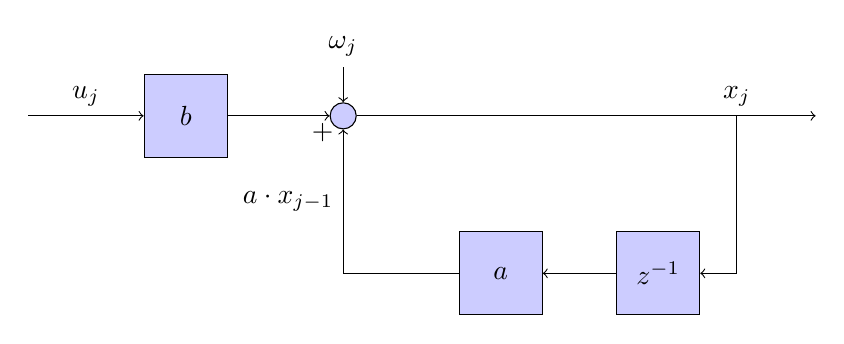
\begin{tikzpicture}[auto, node distance=2cm]
 
	% Input
	\node [input, name=input] {};
 
	% b gain
	\node [block, right of=input] (b) {$b$};
 
	% sum element
	\node [sum, right of=b,
			pin={[pinstyle]above:$\omega_j$},
         	node distance=2cm] (sum) {};
 
	% Two silent nodes in the middle 
	\node [output, right of=sum] (x1) {};
	\node [output, right of=x1] (x2) {};
 
	% Output node
	\node [output, right of=x2] (output) {};
 
	% Nodes in the feedback loop
	\node [block, below of=x2] (delay) {$z^{-1}$};
	\node [block, below of=x1] (a) {$a$};
	
	% Once the nodes are placed, connecting them is easy. 
	\draw [draw,->] (input) -- node {$u_j$} (b);
	\draw [->] (b) -- (sum);
	\draw [-] (sum) -- (x1);
	\draw [-] (x1) -- (x2);
	\draw [->] (x2) -- node [name=y] {$x_j$}(output);
	\draw [->] (y) |- (delay);
	\draw [->] (delay) -- (a);
	\draw [->] (a) -| node[pos=0.99] {$+$} 
     		node [near end] {$a \cdot x_{j-1}$} (sum);
\end{tikzpicture}

\caption{Block diagram illustrating robot position, $x_j$, at discrete time $j$ updated using control action, $u_j$, and the previous position $x_{j-1}$. Stochastic perturbation is introduced using $\omega_j$.}
\end{figure}

Almost always random phenomena are hidden from the observer behind a dynamical system - Kalman described this as follows:\\

\textit{A random function of time may be thought of as the output of a dynamic system excited by an independent Gaussian random process.} \cite{Kalman:1960}\\

This is true for robotic motion, given that we can only attempt to estimate the robot's stochastically perturbed motion, through the use of sensors like odometry, or laser range finders, which are subject to stochastic noise. Letting the measurement of signal $x_j$ be represented by $z_j$, we can write the following equation defining the measurement of $x_j$, subject to noise $\nu_j$, as:
\begin{equation}
z_j = h x_j + \nu_j
\end{equation} 

Equation (2) can be represented in a computational graph as shown in Figure 2.

\newpage

\begin{figure}[h]
\centering
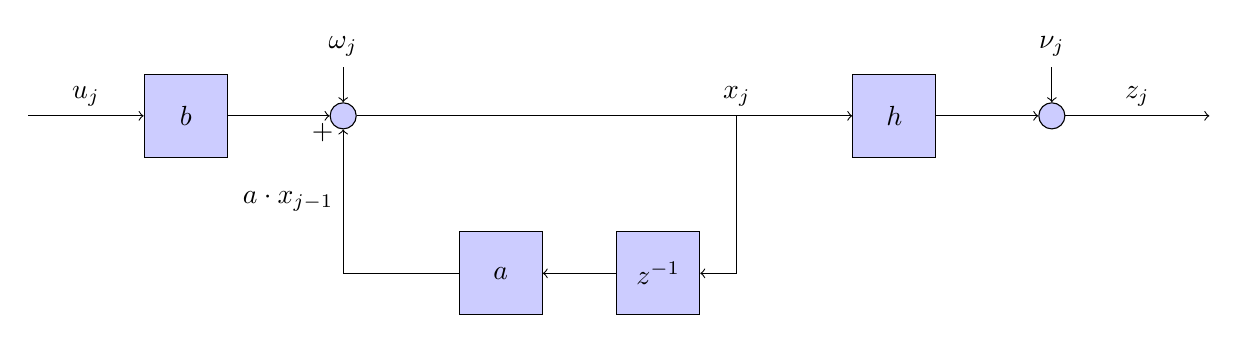
\begin{tikzpicture}[auto, node distance=2cm]

    % Input
    \node [input, name=input] {};
    
    % b gain
    \node [block, right of=input] (b) {$b$};
    
    % sum element
    \node [sum, right of=b,
    pin={[pinstyle]above:$\omega_j$},
            node distance=2cm] (sum) {};
    
    % Two silent nodes in the middle
    \node [output, right of=sum] (x1) {};
    \node [output, right of=x1] (x2) {};
	 
	% Output node
    \node [output, right of=x2] (output) {};
    
    % Nodes in the feedback loop
    \node [block, below of=x2] (delay) {$z^{-1}$};
	\node [block, below of=x1] (a) {$a$};
	
	% Gain on the xj signal
	\node [block, right of=output, node distance=1cm] (h) {$h$};
	
	% sum node
	\node [sum, right of=h,
	    pin={[pinstyle]above:$\nu_j$},
	            node distance=2cm] (sum2) {};
	            
	% measurement output
	\node [output, right of=sum2] (output2) {};
	
    % Once the nodes are placed, connecting them is easy. 
    \draw [draw,->] (input) -- node {$u_j$} (b);
    \draw [->] (b) -- (sum);
    \draw [-] (sum) -- (x1);
    \draw [-] (x1) -- (x2);
    \draw [-] (x2) -- node [name=y] {$x_j$}(output);
    \draw [->] (y) |- (delay);
    \draw [->] (delay) -- (a);
    \draw [->] (a) -| node[pos=0.99] {$+$} 
        node [near end] {$a \cdot x_{j-1}$} (sum);
    
    % measurement section
    \draw [->] (output) -- (h);
    \draw [->] (h) -- (sum2);
    \draw [->] (sum2) -- node [name=y2] {$z_j$}(output2);
\end{tikzpicture}
\caption{Block diagram showing measurement of position, $z_j$. This is an extended iteration of the block diagram shown in Figure 1. Stochastic variance due to imperfect sensors is added with $\nu_j$.}
\end{figure}

The fundamental problem that the Kalman Filter tries to answer is: how can an accurate estimate of a hidden stochastic signal be found when it is observed as the output of a dynamical system? The first step to answering this is to create a mathematical model of the system we can use to find an estimate of the measurement, $z_j$, which we call $\hat{z_j}$. This estimate is based on an estimation of the hidden variable, which we denote with $\hat{x}^-_j$. The mathematical model that provides these estimates does not factor in stochasticity seen in actual signals $x_j$ and $z_j$. This is the \textit{a priori} estimate of $x_j$, and is mathematically described as:
\begin{equation}
\hat{x}^-_j = a \hat{x}_{j-1} + b u_j
\end{equation}

The \textit{a priori} estimate is used to predict an output estimate,  $\hat{z}_j$. In turn, $\hat{z}_j$, is used to estimate the difference between predicted signal and the observed signal, referred to as the residual:
\begin{equation}
z_j - \hat{z}_j = z_j - h \hat{x}^-_j
\end{equation}

If the residual is small, then our estimate is good. If it is large then our estimate is not good. We can use the residual in (4) to update our \textit{a priori} estimate, $\hat{x}^-_j$:
\begin{equation}
\hat{x}_j = \hat{x}^-_j + k (z_j - h \hat{x}^-_j)
\end{equation}

A visualisation of the computational architecture for the process can be seen in Figure 3. This is a useful picture as it allows us to see the Kalman filter process decomposed into two distinct phases:
\begin{enumerate}
\item the state prediction phase in which the residual is used to update the \textit{a priori} providing a state prediction, known as the \textit{posterior belief}
\item the measurement update phase in which the \textit{posterior belief} is updated with control actions $u_j$ and used as the new \textit{a priori}, which is combined with sensor readings to compute the new residual.
\end{enumerate}

\begin{figure}[h]
\centering
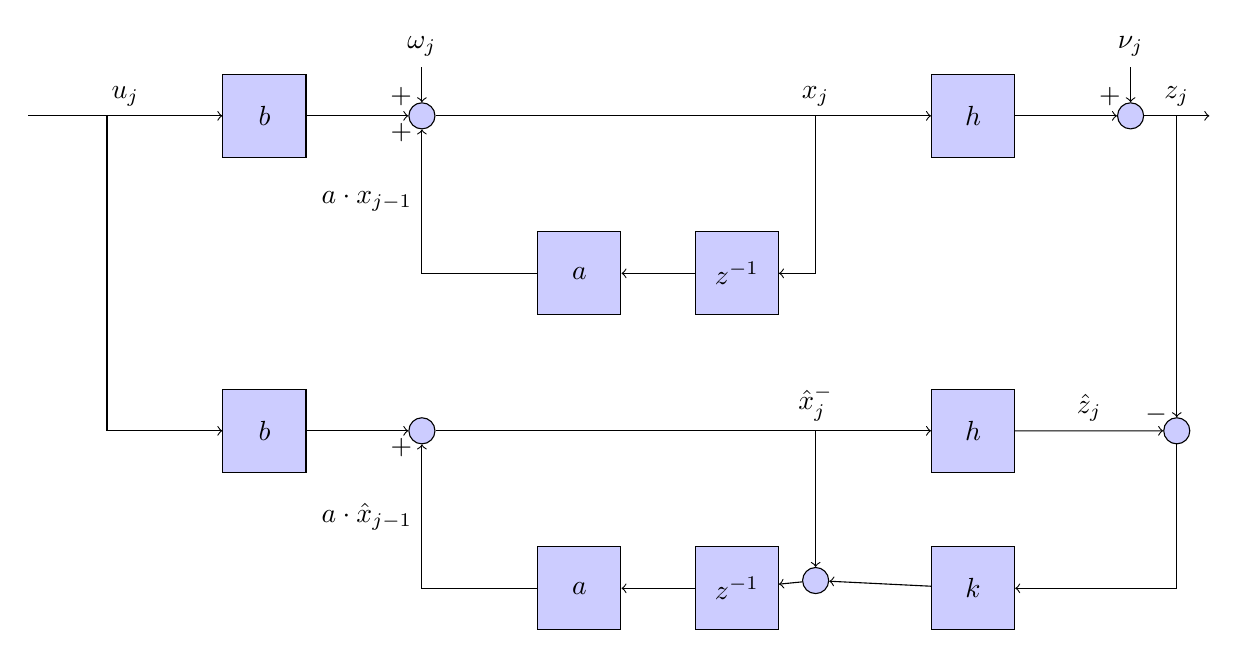
\begin{tikzpicture}[auto, node distance=2cm]
	% % % % % % % % % % % % % % % % % % % % % % %
    % Upper model
    % % % % % % % % % % % % % % % % % % % % % % %
    % Input
    \node [input, name=input] {};
    \node [input, left of=input, node distance=1cm] (start) {};
    
    % b gain
    \node [block, right of=input] (b) {$b$};
    
    % sum element
    \node [sum, right of=b,
    pin={[pinstyle]above:$\omega_j$},
            node distance=2cm] (sum) {};
    
    % Two silent nodes in the middle
    \node [output, right of=sum] (x1) {};
    \node [output, right of=x1] (x2) {};
	 
	% Output node
    \node [output, right of=x2] (output) {};
    
    % Nodes in the feedback loop
    \node [block, below of=x2] (delay) {$z^{-1}$};
	\node [block, below of=x1] (a) {$a$};
	
	% Gain on the xj signal
	\node [block, right of=output, node distance=1cm] (h) {$h$};
	
	% sum node
	\node [sum, right of=h,
	    pin={[pinstyle]above:$\nu_j$},
	            node distance=2cm] (sum2) {};
	            
	% measurement output
	\node [output, right of=sum2, node distance=1cm] (output2) {};
	
    % Once the nodes are placed, connecting them is easy. 
    %\draw [draw,->] (start) -- (input);
    \draw [draw,->] (start) -- node {$u_j$} (b);
    \draw [->] (b) -- node[pos=0.93] {$+$} (sum);
    \draw [-] (sum) -- (x1);
    \draw [-] (x1) -- (x2);
    \draw [-] (x2) -- node [name=y] {$x_j$}(output);
    \draw [->] (y) |- (delay);
    \draw [->] (delay) -- (a);
    \draw [->] (a) -| node[pos=0.99] {$+$} 
        node [near end] {$a \cdot x_{j-1}$} (sum);
    
    % measurement section
    \draw [->] (output) -- (h);
    \draw [->] (h) -- node[pos=0.93] {$+$} (sum2);
    \draw [->] (sum2) -- node [name=y2] {$z_j$}(output2);
    
    
    % % % % % % % % % % % % % % % % % % % % % % %
    % Lower model
    % % % % % % % % % % % % % % % % % % % % % % %
    
    % lower b node
    \node [block, below of=b, node distance=4cm] (be) {$b$};
    
    % sum element
    \node [sum, right of=be, node distance=2cm] (sume) {};
        
    % Two silent nodes in the middle
    \node [output, right of=sume] (x1e) {};
    \node [output, right of=x1e] (x2e) {};
    	 
    % Output node
    \node [output, right of=x2e] (outpute) {};
        
    % Nodes in the feedback loop
    \node [block, below of=x2e] (delaye) {$z^{-1}$};
    \node [block, below of=x1e] (ae) {$a$};
    
    % Gain on the xj signal
    \node [block, right of=outpute, node distance=1cm] (he) {$h$};
    		            
    % measurement output
    \node [output, right of=he] (output2e) {};
    
    \node [sum, below of=y2, node distance=4.25cm] (sum2e) {};
    
    \node [block, below of=he] (k) {$k$};
    
    % Once the nodes are placed, connecting them is easy.
    \draw [->] (input) |- (be);
    \draw [->] (be) -- (sume);
    \draw [-] (sume) -- (x1e);
    \draw [-] (x1e) -- (x2e);
    \draw [-] (x2e) -- node [name=ye] {$\hat{x}^-_j$}(outpute);
    %\draw [->] (ye) |- (delaye);
    \draw [->] (delaye) -- (ae);
    \draw [->] (ae) -| node[pos=0.99] {$+$} 
            node [near end] {$a \cdot \hat{x}_{j-1}$} (sume);
        
    % measurement section
    \draw [->] (outpute) -- (he);
    \draw [->] (he) -- node [name=y2e] {$\hat{z}_j$}(sum2e);
    
    \draw [->] (y2) -- node[left, pos=0.99] {$-$} (sum2e);
    
    \node [sum, below of=ye, node distance=2.25cm] (sumfin) {};
    
    \draw [->] (sum2e) |- (k);
    \draw [->] (ye) -- (sumfin);
    \draw [->] (k) -- (sumfin);
    \draw [->] (sumfin) -- (delaye);
    
\end{tikzpicture}
\caption{Block diagram showing the actual measurement model (above), and the prediction model (below). The outputs of the two models are compared and fed to a feedback topology. Core to the Kalman filter implementation is the selection of weights $k$ in the bottom right hand corner.}
\end{figure}

The task of determining $k$, used to refine our estimate, is at the heart of the Kalman filtering process. This is not a trivial task. Further, our problem is complicated when considering robotic motion in multiple dimensions - so far, estimation has only been considered for a 1D problem. Most mobile robots move in 2D, and we may also want to estimate other important locomotion variables such as velocity. Suppose that state was now represented as vector of variables such as position in 2D, including velocity. We define this using bold typeface $\mathbf{x}_j$. Similarly, control actions are represented as $\mathbf{u}_j$, and the measurement for each state variable in $\mathbf{x}_j$ is represented by $\mathbf{z}_j$. Without loss of generality equation (1) becomes:
\begin{equation}
\mathbf{x}_j = \mathbf{A} \mathbf{x}_j + \mathbf{B} \mathbf{u}_j + \boldsymbol{\omega}_j
\end{equation}

Similarly, equation (2) becomes:
\begin{equation}
\mathbf{z}_j = \mathbf{H} \mathbf{x}_j + \boldsymbol{\nu}_j
\end{equation}

The \textit{a priori} estimate of the state variable, shown in equation (3), in multidimensional form, is given by:
\begin{equation}
\hat{\mathbf{x}}^-_j = \mathbf{A} \hat{\mathbf{x}}_j + \mathbf{B} \mathbf{u}_j
\end{equation}

The \textit{a priori} update, shown in equation (5) is given by:
\begin{equation}
\hat{\mathbf{x}}_j = \hat{\mathbf{x}}^-_j + \mathbf{K}_j (\mathbf{z}_j - \mathbf{H} \hat{\mathbf{x}}^-_j)
\end{equation}

The error for the \textit{posterior}, $\mathbf{e}_j$, can be written as:
\begin{equation}
\mathbf{e}_j = \mathbf{x}_j - \hat{\mathbf{x}}_j
\end{equation}

A common way to measure the accuracy of $\mathbf{e}_j$ is using the covariance matrix, denoted in the literature as $\mathbf{P}_j$. This can be expressed as follows:
\begin{equation}
\mathbf{P}_j = \mathbb{E}[\mathbf{e}_j \cdot \mathbf{e}_j]
\end{equation}

The Kalman filter attempts to select the Kalman Filter gain, $\mathbf{K}$, such that the \textit{posterior} covariance is minimised. Applying a classical optimisation technique for multivariate calculus, we arrive at the following expression:
\begin{equation}
\frac{\partial \mathbf{P}_j}{\partial \mathbf{K}_j} = \frac{\partial \mathbb{E}[(\mathbf{x}_j - \hat{\mathbf{x}}_j)(\mathbf{x}_j - \hat{\mathbf{x}}_j)^T]}{\partial \mathbf{K}_j} = 0
\end{equation}

Solving equation (12) yields the following result for the Kalman filter gain:
\begin{equation}
\mathbf{K}_j = \frac{\mathbf{P}_j \mathbf{H}^T}{\mathbf{H} \mathbf{P}_j \mathbf{H}^T + \mathbf{R}}
\end{equation}

The denominator of equation (13) contains the measurement noise, represented by matrix $\mathbf{R}$. In fact, the denominator is an important calculation step that maps the state prediction covariance, $\mathbf{P}_j$, into the measurement space - often this is expressed with the variable $\mathbf{S}$, that is:
\begin{equation}
\mathbf{S} = \mathbf{H} \mathbf{P}_j \mathbf{H}^T + \mathbf{R} 
\end{equation}

In addition to the \textit{posterior} error, $\mathbf{e}_j$, there is an error for the \textit{a priori}, denoted $\mathbf{e}^-_j$. The covariance matrix for $\mathbf{e}^-_j$ is given by $\mathbf{P}^-_j$. The final step to arriving at an algorithm for the Kalman filter is being able to recursively update both the \textit{posterior} and \textit{a priori} covariance matrices. The \textit{a priori} error covariance update is derived from considering the error expression $\mathbf{x}_j - \hat{\mathbf{x}}^-_j$, and is expressed using the movement noise matrix $\mathbf{Q}$. The expression is as follows:
\begin{equation}
\mathbf{P}^-_j = \mathbf{A} \mathbf{P}_{j-1} \mathbf{A}^T + \mathbf{Q}
\end{equation}

The \textit{posterior} update can be derived from equation (11), and is expressed as:
\begin{equation}
\mathbf{P}_j = (\mathbf{I} - \mathbf{K}_j \mathbf{H}) \mathbf{P}^-_j
\end{equation}

Equations (8), (9), (13), (14), (15), and (16) make up the Kalman Filter algorithm. A single pass of the Kalman Filter algorithm can be seen in Algorithm 1 - the pass starts with the \textit{a priori} state estimate update, and concludes with the \textit{posterior} error covariance update. The full algorithm would see the code run continuously, in a loop, iteratively updating state and covariance estimations.
\begin{algorithm}
\caption{Kalman Filter}
\begin{algorithmic}[1]
\State $\hat{\mathbf{x}}' \gets \mathbf{A} \hat{\mathbf{x}} + \mathbf{B} \mathbf{u}$ (A Priori State Estimate Update)
\State $\mathbf{P}' \gets \mathbf{A} \mathbf{P} \mathbf{A}^T + \mathbf{Q}$ (A Priori Error Covariance Update)
\State $\mathbf{S} \gets \mathbf{H} \mathbf{P}' \mathbf{H}^T + \mathbf{R}$ (Covariance Update In Measurement Space)
\State $\mathbf{K} \gets \mathbf{P}' \mathbf{H}^T \mathbf{S}^{-1}$ (Kalman Gain Update)
\State $\mathbf{x} \gets \mathbf{x}' + \mathbf{K}(\mathbf{z} - \mathbf{H} \mathbf{x}')$ (Posterior State Estimate Update Using Kalman Gain)
\State $\mathbf{P} \gets (\mathbf{I} - \mathbf{K} \mathbf{H}) \mathbf{P}'$ (Posterior Error Covariance Update)
\end{algorithmic}
\end{algorithm}

NEED TO TALK ABOUT EXTENDED KALMAN FILTER

\subsection{Particle Filters}
Particle filters can be used to solve the global localisation problem, that is, it can localise a robot in an environment when its initial position is unknown. This section looks at a specific type of particle filter known as Monte Carlo Localisation (MCL). The central idea of MCL is the estimation of a posterior distribution across robot poses, often referred to as the \textit{belief}. The \textit{belief} is defined as probability density over the pose state space, which is conditioned on sensor measurement data, and odometric action data. Mobile robot pose, $\mathbf{x}$, is made up of location coordinates $x$ and $y$ and orientation $\theta$. Letting observation from a laser range finder be represented by $\mathbf{z}$, and odometric sensor data by represented by $\mathbf{u}$, we can mathematically express the belief as follows:
\begin{equation}
Bel(\mathbf{x}_t) = p(\mathbf{x}_t | \mathbf{z}_t, \mathbf{u}_{t-1}, \mathbf{z}_{t-1}, \mathbf{u}_{t-2},\ldots,\mathbf{z}_0)
\end{equation}

Particle filters estimate belief recursively, meaning that an update rule from time $t$ to time $t+1$ is required, and an initial belief is also needed. The initial belief characterizes the initial knowledge about the system state - if little is known about the initial system state, then a uniform distribution can be used over the state space. To derive the update equation we start by expressing (17) using Bayes rule:
\begin{equation}
Bel(\mathbf{x}_t) = \frac{p(\mathbf{z}_t | \mathbf{x}_t,\mathbf{u}_{t-1},\ldots,\mathbf{z}_0) \ p(\mathbf{x}_t | \mathbf{u}_{t-1},\ldots,\mathbf{z}_0)}{p(\mathbf{z}_t | \mathbf{u}_{t-1},\ldots,\mathbf{z}_0)}
\end{equation}

The denominator is a constant value relative to $\mathbf{x}_t$, and (4) can be written more compactly as:
\begin{equation}
Bel(\mathbf{x}_t) = \eta \ p(\mathbf{z}_t | \mathbf{x}_t,\mathbf{u}_{t-1},\ldots,\mathbf{z}_0) \ p(\mathbf{x}_t | \mathbf{u}_{t-1},\ldots,\mathbf{z}_0)
\end{equation}

where $\eta$ is a constant value:
\begin{equation}
\eta = p(\mathbf{z}_t | \mathbf{u}_{t-1},\ldots,\mathbf{z}_0)^{-1}
\end{equation}

A recursive relation seeks to provide an update at each time step. Information from the past is factored into the belief as changes occur. Therefore it can be reasoned that only new information presented to the system from current state is important when modifying the belief. This simplifying assumption, referred to as the \textit{Markov assumption}, suggests that future data is independent of past data given knowledge of the current state. Mathematically, this allows equation (5) to be re-written as:
\begin{equation}
Bel(\mathbf{x}_t) = \eta \ p(\mathbf{z}_t | \mathbf{x}_t) \ p(\mathbf{x}_t | \mathbf{u}_{t-1},\ldots,\mathbf{z}_0)
\end{equation} 

Partitioning over $\mathbf{x}_{t-1}$ equation (7) can be written as:
\begin{equation}
Bel(\mathbf{x}_t) = \eta \ p(\mathbf{z}_t | \mathbf{x}_t) \int p(\mathbf{x}_t, \mathbf{x}_{t-1} | \mathbf{a}_{t-1},\ldots,\mathbf{z}_0) \ d\mathbf{x}_{t-1}
\end{equation}

Applying Bayes' equation (8) can be written as:
\begin{equation}
Bel(\mathbf{x}_t) = \eta \ p(\mathbf{z}_t | \mathbf{x}_t) \int p(\mathbf{x}_{t} | \mathbf{x}_{t-1},\mathbf{u}_{t-1},\ldots,\mathbf{z}_0) \ p(\mathbf{x}_{t-1} | \mathbf{u}_{t-1},\ldots,\mathbf{z}_0) \ d\mathbf{x}_{t-1}
\end{equation}

Exploiting the Markov property again the first expression in the integral can be simplified. The second expression can be written using the $Bel$ notation as follows:
\begin{equation}
Bel(\mathbf{x}_t) = \eta \ p(\mathbf{z}_t | \mathbf{x}_t) \int p(\mathbf{x}_{t} | \mathbf{x}_{t-1},\mathbf{u}_{t-1}) \ Bel(\mathbf{x}_{t-1}) \ d\mathbf{x}_{t-1}
\end{equation}

There are two key components to equation (10):  the first is probability $p(\mathbf{x}_t| \mathbf{x}_{t-1}, \mathbf{u}_{t-1})$ which is referred to as the \textit{motion model}; and the second is the probability $p(\mathbf{z}_t|\mathbf{x}_t)$ which is referred to as the \textit{sensor model}.

\subsubsection{Motion model $p(\mathbf{x}_t| \mathbf{x}_{t-1}, \mathbf{u}_{t-1})$ and sensor model $p(\mathbf{z}_t|\mathbf{x}_t)$}
Under noise free ideal conditions the robot moves from state $\mathbf{x}_{t-1}$ to state $\mathbf{x}_t$ with certainty given some control action $\mathbf{u}_{t-1}$ - the assumption of idealness allows the use of kinematic equations to fully describe the robot's motion. As previously discussed, however, physical robot motion is subject to uncertainty since actuators are not ideal, which means there is uncertainty in pose $mathbf{x}_{t}$. The \textit{motion model}, $p(\mathbf{x}_t| \mathbf{x}_{t-1}, \mathbf{u}_{t-1})$, describes a posterior density over successors to pose $\mathbf{x}_{t-1}$. A graphical depiction of what this looks like can be seen in Figure XXXX, which shows the distribution over where the robot could be located given some control action. The image on the right shows the distribution of the robot location after moving 40 meters. The picture on the right shows a more complicated path. The darker regions of the distribution indicate more likely robot locations. 

\begin{figure}[h]
\centering
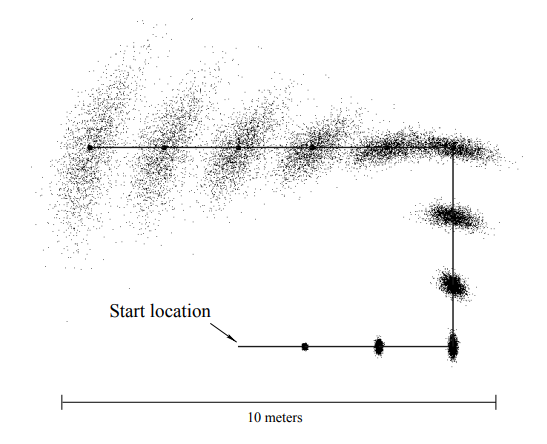
\includegraphics[scale=0.4]{motion_model}
\caption{As the robot moves from the start location we see that the uncertainty of where the robot is located increases. This uncertainty is described by the \textit{motion model} - dispersed dots indicate higher uncertainty.}
\end{figure}

The sensor model provides the probability, or likelihood, of obtaining the sensor measurements, $\mathbf{z}_t$, given a robot pose, $\mathbf{x}_t$ and control action $\mathbf{u}_{t-1}$, assuming that we have a known map. Sensors such as laser range finders are made up of multiple beams.

\subsubsection{MCL Implementation}
The state space for mobile robot localisation is continuous, meaning that implementing the recursive localisation equation shown in (24) is computationally intractable. Particle filter algorithms attempt to represent the belief $Bel(\mathbf{x}_t)$ using a set of $m$ weighted samples distributed according to $Bel(\mathbf{x}_t)$. Mathematically, we can express this as:
\begin{equation}
Bel(\mathbf{x}_t) \approx \{\mathbf{x}^{(i)}, \omega^{(i)} \}_{i=1,...,m}
\end{equation}

The sampled particles, $\mathbf{x}^{(i)}$, are discrete hypotheses of the robot's pose drawn from $Bel(\mathbf{x}_t)$. The $\omega^{(i)}$, called the \textit{importance factor}, are derived based on how likely the hypothesis particle is, given the sensor measurements and known map. The idea is that over time the set of sample particles converge on the true robot pose in the environment. This means that the algorithm needs to discard particles that are unlikely, and keep particles that are likely. Indeed the MCL algorithm can be thought of as featuring two distinct components:
\begin{enumerate}
\item \textbf{Motion and sensor update}: this phase sees the robot undergo a control action which is applied to its pose, as well as the pose of all particles. Additionally, sensor measurements are obtained, and then these sensor readings are used to determine new likelihood weights, $\omega$, for each of the particles.
\item \textbf{Resampling}: this phase allows us to discard particles which are not likely (low weights), and keep particles with high likelihood (i.e. large weights). This is undertaken by randomly sampling $m$ times from the pool of particles, with replacement. Higher $\omega$ weights mean it is more likely the particle will feature in the re-sampled set.
\end{enumerate}

The MCL algorithm pseudocode is shown in Algorithm 2 below.
\begin{algorithm}
\caption{Monte Carlo Localisation}
\begin{algorithmic}[1]
\Procedure{MCL}{$X_{t-1}$,$u_t$,$z_t$}
\State $\bar{X}_t = X_T = \emptyset$
\For{$m=1$ to $M$}
	\State $x^{[m]}_t = \text{motion\_update}(u_t, x^{[m]}_{t-1})$
	\State $\omega^{[m]}_t = \text{sensor\_update}(z_t, x^{[m]}_t)$
\EndFor
\For{$m=1$ to $M$}
	\State $\text{draw} \ x^{[m]}_t \ \text{from} \  \bar{X}_t \ \text{with probability} \propto \omega^{[m]}_t$
	\State $X_t = X_t + x^{[m]}_t$
\EndFor
\State $\text{return} \ X_t$
\EndProcedure
\end{algorithmic}
\end{algorithm}

\subsection{Comparison \& Model Selection}
Kalman filters and MCL present very different approaches to solving the localisation problem. Kalman filters make underlying assumptions about the distribution of stochastic perturbation to model actuation and sensor noise in order to predict true robot pose - it assumes Gaussian distributions. As a result the pose posterior is also Gaussian. In contrast, MCL does not make this restrictive assumption and instead takes samples using particles to estimate the pose distribution. This means that the MCL is more robust than a Kalman filter approach given that it can handle situations in which there are violations of distribution assumptions in KF. The principal drawback of MCL is that it is much more expensive in terms of memory requirements and computational processing. This is because to properly estimate the pose distribution a large number of samples (particles) need to be stored and updated for each discrete time step in the algorithm. The main advantage of MCL over a Kalman filter approach is that it can recover from wheel slip events, that is, the MCL algorithm can solve the global localisation problem, whereas a Kalman filter can only be used for position tracking. MCL was selected to implement in simulation, given that it is able to solve the global localisation problem making it a more robust solution.

\newpage

\section{Simulations}
Gazebo, a physical simulation environment, was used to test an off-the-shelf implementation of MCL on two mobile robot platforms: a benchmark model, and a personal model. ROS was used to implement and run the various process nodes which make up the robot model, and RVIZ was used to visualise sensor data, costmaps, and navigation paths. A basic simulated environment was used to test MCL performance for spawned robots - map topology can be seen in Figure XXXX.
\begin{figure}[h]
\centering
\frame{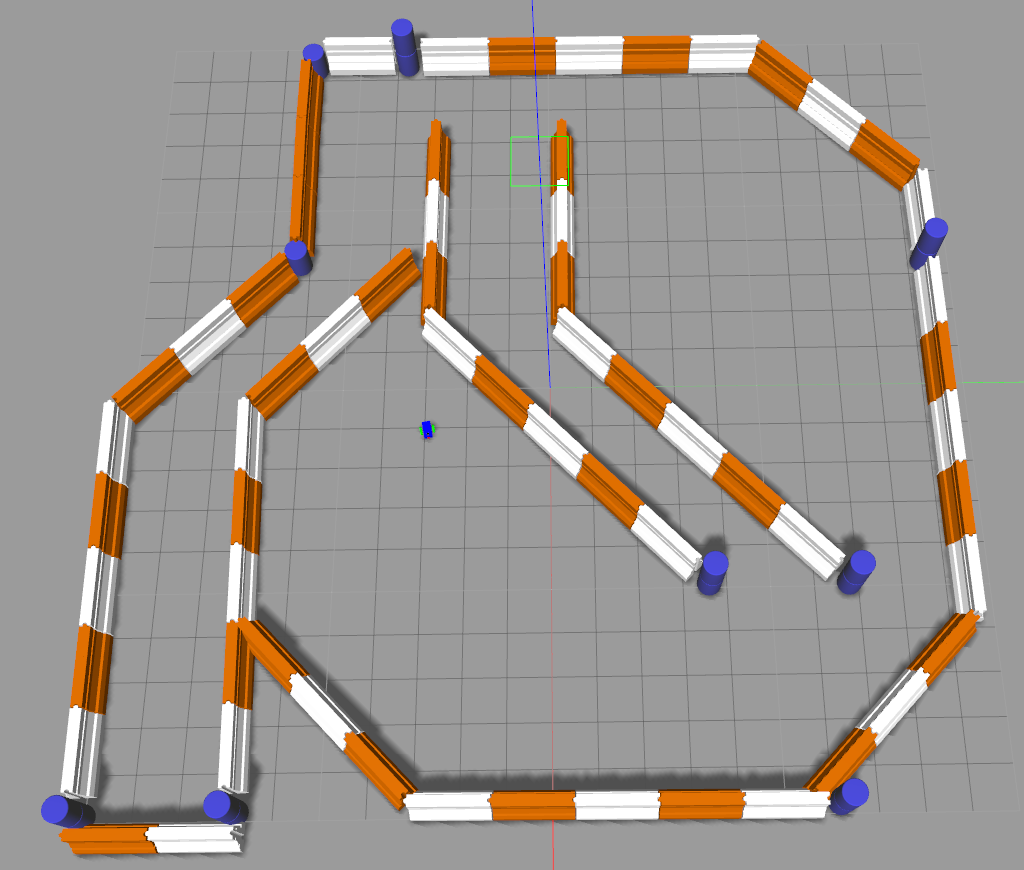
\includegraphics[scale=0.35]{map_topology}}
\caption{Simple environment topology was used to test the robot model MCL performance}
\end{figure}

The benchmark robot model was designed for easy implementation of the MCL package with ROS, Gazebo, and RVIZ. The second robot model, based heavily on the benchmark model, was designed to assess how different physical sensor locations impact MCL performance. Further, modifications were made to the physical robot body to determine if robot chassis geometries affect MCL performance. To evaluate MCL performance, each robot was provided an identical goal pose (location and orientation). Robots had to localise in the environment, and navigate to the goal pose. Performance metrics included: time taken to localise; and time taken to reach goal pose.

\subsection{Benchmark Model}
\subsubsection{Model Design}
The benchmark robot model consisted of a rectangular prism chassis, along with two cylindrical wheels placed in a differential drive configuration in the middle of the chassis. Frictionless, semi-spherical, casters were placed in symmetrical locations on either end of the chassis to ensure stability. A camera, modelled with a red cube, was placed on the front of the chassis. A laser range finder was placed on top of the chassis, towards the camera location.
\begin{figure}[h]
\centering
\frame{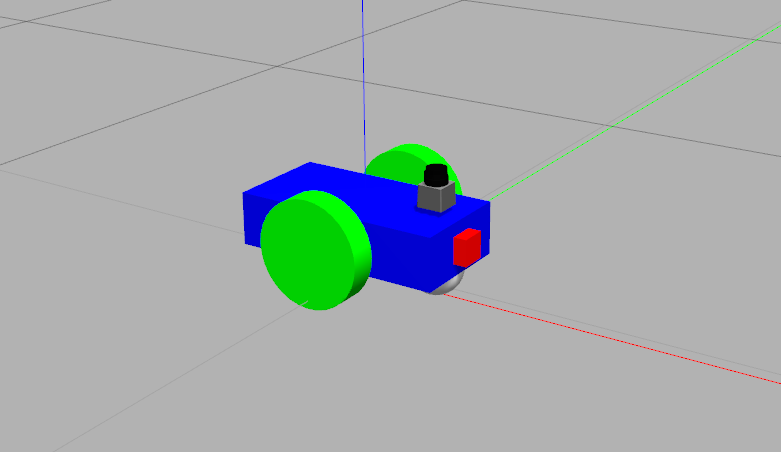
\includegraphics[scale=0.37]{benchmark_model}}
\caption{Benchmark robot model is comprised of a rectangular prism chassis, and two wheels arranged in a differential drive configuration on either side of the chassis. The chassis is equipped with a front mounted RGB camera, and a laser range finder. Frictionless casters provide stability underneath the chassis.}
\end{figure}

\begin{minipage}{0.45\textwidth}
Figure XXXX shows the robot model loaded into an empty world using Gazebo. The robot was equipped with a differential drive controller, called \texttt{libgazebo\_ros\_diff\_drive.so}, which allowed ROS to control the robot wheels. Similarly, controllers for the camera and laser range finder were equipped which were called \texttt{libgazebo\_ros\_camera.so} and \texttt{libgazebo\_ros\_laser.so}, respectively. The robot dimensions can be seen in Table XXXX.
\end{minipage}
\hspace{1cm}
\begin{minipage}{0.45\textwidth}
\centering
\captionof{table}{Descriptive measurement summary for the benchmark model}
\begin{tabular}{lc}
\toprule
\textbf{Dimension} & \textbf{Measurement ($\si{\meter}$)} \\
\midrule
Chassis Length & 0.4\\
Chassis Width & 0.2\\
Chassis Height & 0.1\\
Wheel Radius & 0.1\\
Wheel Placement & Center\\
\bottomrule
\end{tabular}
\end{minipage}


\subsubsection{Personal Model}
An alternative model was developed by modifying the benchmark design. The original chassis was retained, however, the cylindrical wheels were shifted to the rear, in a differential drive configuration. Two frictionless semi-spherical casters were set symmetrically at either end of the chassis. The camera was left in its original location.
\begin{figure}[h]
\centering
\frame{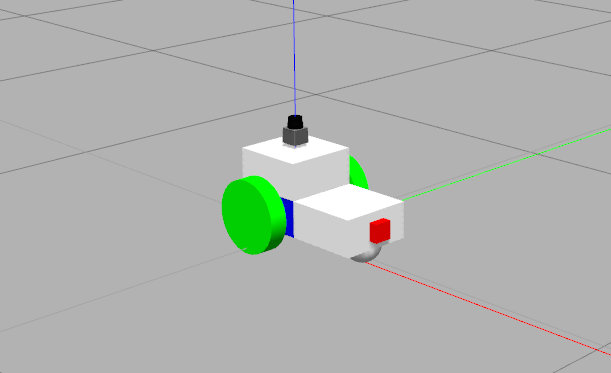
\includegraphics[scale=0.47]{shane_model}}
\caption{Personal robot model is comprised of a rectangular prism chassis, and two wheels arranged in a differential drive configuration towards the chassis rear. The model is equipped with a front mounted RGB camera, and a laser range finder. Frictionless casters provide stability underneath the chassis.}
\end{figure}

\begin{minipage}{0.45\textwidth}
To provided an elevated location for the laser range finder the height of the robot chassis at the rear was elevated. Figure XXXX shows the robot model loaded into an empty world using Gazebo. The robot was equipped with controllers for the differential drive, camera, and laser range finder identical to the benchmark model. Dimensions can be seen in Table XXXX.
\end{minipage}
\hspace{1cm}
\begin{minipage}{0.45\textwidth}
\centering
\captionof{table}{Descriptive measurement summary for the personal model}
\begin{tabular}{lc}
\toprule
\textbf{Dimension} & \textbf{Measurement ($\si{\meter}$)} \\
\midrule
Chassis Length & 0.4\\
Chassis Width & 0.2\\
Chassis Height & 0.1\\
Wheel Radius & 0.1\\
Wheel Placement & Rear\\
\bottomrule
\end{tabular}
\end{minipage}

\newpage

\subsection{Packages}
Two main packages are required to implement MCL in simulation. The first is the \texttt{amcl} package - an MCL package that alters the number of particles used to improve algorithm efficiency. The second package is the \texttt{move\_base} package which is used to generate cost maps and navigation paths for the robot model to reach goal locations. Sections 3.2.1 and 3.2.2 discuss the \texttt{amcl} and \texttt{move\_base} packages, respectively.

\subsubsection{\texttt{amcl} package}
The \texttt{amcl} package is a localisation system for a robot traversing 2D map topologies, which is implemented in ROS. The package implements an Monte Carlo localisation approach that uses a particle filter to track the pose of the robot for a given known map. Unlike standard MCL algorithms, this package implements an adaptive filter, which changes the number of sampled particles dynamically to ensure that error introduced by the sample-based representation is bounded.

Some of the more important parameters for this package include:
\begin{itemize}
\item \textbf{\texttt{min\_particles}} and \textbf{\texttt{max\_particles}}: amcl dynamically adjusts the number of particles for each iteration, between some given range. A range with a high maximum may be too computationally expensive, for a given system.
\item \textbf{\texttt{update\_min\_a}} and \textbf{\texttt{update\_min\_d}}: upon receiving a laser scan, amcl checks the linear and angular displacement of the robot from the last laser scan and will only provide a filter update if these values are greater than the values specified in these parameters 
\item \textbf{\texttt{transform\_tolerance}}: the duration for which a published transform is valid
\item \textbf{\texttt{laser\_min\_range}} and \textbf{\texttt{laser\_max\_range}}: define the minimum and maximum scan ranges that will be considered for the laser range finder 
\item \textbf{\texttt{laser\_max\_beams}}: how many evenly spaced beams in each scan to be used when updating the filter
\end{itemize}

\subsubsection{\texttt{move\_base} package}
The \texttt{move\_base} package provides the robot with a navigation and path planning tool. Given a goal in the world, the \texttt{move\_base} package will provide action to reach it with a mobile base. This is comprised of a global path planner, and a local path planner. The \texttt{mve\_base} node, once initialised, will also maintain two costmaps: one for the global planner, and one for the local planner. These maps are integral to accomplish navigation tasks. The \texttt{move\_base} node subscribes to a number of different topics. These include:
\begin{itemize}
\item an environment map provided by a map server;
\item laser scans from a laser range finder;
\item point cloud data from RGBD cameras;
\item odometric data from the robot odometry;
\item sensor transforms from a transform topic; and
\item transform updates from amcl nodes
\end{itemize}

The \texttt{move\_base} node receives a simple goal pose, and outputs a series of commands to the robot's base controller in order to achieve the input goal. The visual graph depicting the navigation stack set up can be seen in Figure XXXX.
\begin{figure}[h]
\centering
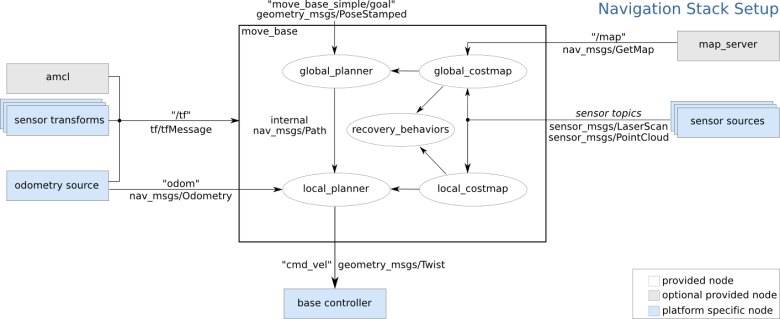
\includegraphics[scale=0.7]{move_base}
\caption{A depiction of the navigation stack used to localise the robot in a known environment using and MCL implementation. The \texttt{move\_base} node subscribes to the output of the \texttt{amcl} node. Additionally, a map server provides \texttt{move\_base} with a ground truth map. The \texttt{move\_base} node also receives odometry and sensor data, and provides output to the control node.}
\end{figure}

Some of the more important parameters for this package include:
\begin{itemize}
\item \textbf{\texttt{controller\_frequency}}: the rate in $\si{\hertz}$ at which to run the control loop and send velocity commands to the base
\item \textbf{\texttt{update\_frequency}}: the frequency in $\si{\hertz}$ for the map to be updated
\item \textbf{\texttt{publish\_frequency}}: the frequency in $\si{\hertz}$ for the map to be published
\item \textbf{\texttt{inflation\_radius}}: the radius in meters to which the map inflates obstacle cost values
\item \textbf{\texttt{obstacle\_range}}: the maximum range in meters at which to insert obstacles into the costmap using sensor data
\item \textbf{\texttt{raytrace\_range}}: the maximum range in meters at which to raytrace out obstacles from the map using sensor data
\end{itemize}

\subsection{Parameter Tuning}
\begin{minipage}{0.55\textwidth}
Parameters were tuned for the benchmark model using trial and error. This undertaken iteratively until a set of parameters were found allowing error free movement over short linear distances. Parameters were tuned one at a time by entering a test value for the model configuration, and then loading the model into the world, with an active \texttt{amcl} and \texttt{move\_base} node. Desired poses were provided a short distance from the original pose, and performance was evaluated visually. This process was continued until satisfactory localisation and navigation behaviours emerged for the benchmark model - the tuned parameter values can be seen in Table 1.
\end{minipage}
\hspace{0.75cm}
\begin{minipage}{0.35\textwidth}
\centering
\captionof{table}{Parameter value summary for \texttt{amcl}, and \texttt{move\_base}}
\begin{tabular}{lr}
\toprule
\textbf{Parameter} & \textbf{Value}\\
\midrule
\texttt{controller\_frequency} & 10.0 \\
\texttt{update\_frequency} & 20.0 \\
\texttt{publish\_frequency} & 20.0 \\
\texttt{transform\_tolerance} & 0.2 \\
\texttt{inflation\_radius} & 0.3 \\
\texttt{obstacle\_range} & 8.0\\
\texttt{raytrace\_range} & 10.0\\
\bottomrule
\end{tabular}
\end{minipage}



\section{Results}
Robot models were deployed separately in the environment using identical parameter configurations for their \texttt{move\_base} and \texttt{amcl} nodes. Both models successfully generated a costmap, which was used for navigation. The physical environment, the ground truth map, and the local costmap, for the benchmark model, can be seen in Figures XXXX, XXXX, and XXXX, respectively. Robots, provided with a goal pose, were required to localise in the environment and navigate to the goal pose. Successful localisation saw particle convergence around the correct robot pose, which was determined by visual inspection. Time taken to localise, and time taken to reach the goal were measured. Each robot underwent five separate trials.\\

\begin{minipage}[t]{0.45\textwidth}
\centering
\frame{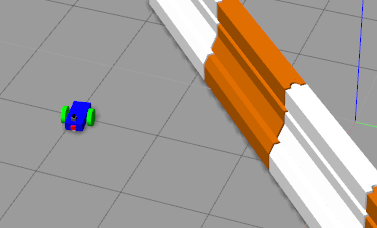
\includegraphics[height=4cm]{cost_map_1}}
\captionof{figure}{Actual physical environment. The robot is located near a barrier in the environment.}
\end{minipage}
\hspace{1cm}
\begin{minipage}[t]{0.45\textwidth}
\centering
\frame{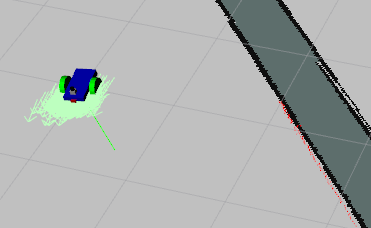
\includegraphics[height=4cm]{cost_map_2}}
\captionof{figure}{The ground truth map which is provided to \texttt{move\_base} via a map server node.}
\end{minipage}

\vspace{0.25cm}

\begin{minipage}{0.45\textwidth}
The benchmark model was able to localise in all five trials and avoided collisions with environment obstacles. The robot became stuck in two trials, and was unable to recover. Interestingly, the robot did not get stuck on the environment obstacles, rather, it became stuck on an \textit{invisible} barrier. The remaining three trials saw the robot successfully navigate to the desired goal pose. The average localisation time over the three successful trials was 0.49 seconds, and the average time to goal was 1 minute and 36 seconds. The full set of results can be seen in Table XXXX.
\end{minipage}
\hspace{1cm}
\begin{minipage}{0.45\textwidth}
\centering
\frame{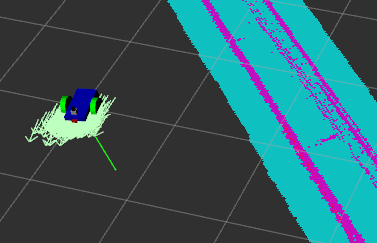
\includegraphics[height=4cm]{cost_map_3}}
\captionof{figure}{A local costmap generated by the \texttt{move\_base} node inflates objects to help avoid collisions.}
\end{minipage}

\vspace{0.5cm}

The personal model as able to localise in all five trials and avoided collisions with environment obstacles. The robot became stuck in three trials, and was unable to recover. As with the benchmark model, the robot did not become stuck on actual physical obstacles. The remaining three trials saw the robot successfully navigate to the desired goal pose. The average localisation time over two successful trials was 0.375 seconds, and the average time to goal was 1 minute and 21 seconds. The full set of results can be seen in Table XXXX.

\begin{table}[h]
\centering
\caption{Five independent trials in which the robot was required to navigate to a given goal pose for benchmark and personal models. Listed results show the time taken to localise and the time taken reach goal pose.}
\begin{tabular}{crrcrr}
\toprule
& \multicolumn{2}{c}{\textbf{Benchmark Model}} & & \multicolumn{2}{c}{\textbf{Personal Model}} \\
\cline{2-3} \cline{5-6}
\textbf{Trial} & \textbf{Localisation} & \textbf{Goal} & & \textbf{Localisation} & \textbf{Goal} \\
\midrule
1 & 0.48 & 1.36 & & \texttt{stuck} & \texttt{stuck} \\
2 & 0.47 & 1.36 & & \texttt{stuck} & \texttt{stuck} \\
3 & \texttt{stuck} & \texttt{stuck} & & \texttt{stuck} & \texttt{stuck} \\
4 & 0.52 & 1.37 & & 0.39 & 1.21 \\
5 & \texttt{stuck} & \texttt{stuck} & & 0.36 & 1.21 \\
\bottomrule
\end{tabular}
\end{table}

Benchmark model performance, during a successful run, can be seen in Figures 12, 14. and 16. Figure XXXX shows the benchmark model initialised in the environment. The green arrows represent the distribution of particles used by the \texttt{amcl} node. Note they are uniformly distributed around the robot. Figure XXXX shows the robot navigating towards the goal location - the green arrows are starting to converge on the robots true pose within the environment map. Finally, Figure XXXX shows the robot at the goal pose. The arrows are tightly clustered around the robot demonstrating that \texttt{amcl} has localised the robot within the environment. Figures XXXX, XXXX, and XXXX show the same sequence of events for the personal robot model on a successful run.

\section{Discussion}
The benchmark model appears the most stable as it was able to navigate the goal pose more reliably than the personal model. It must be noted, however, that this may simply be an artefact of the stochastic initialisation and pose evolution of the particles that are used in the \texttt{amcl} node. The \texttt{amcl} node randomly initialises the distribution of particles, and each discrete time step adds random perturbations to particle movement, and sensor measurements. Given that the \texttt{amcl} outputs to the \texttt{move\_base} node, it may be the case that both models are equally likely to get stuck - more trials need to be undertaken to determine if both models are equally likely to get stuck. No immediate reason is presented as to why the robot models are getting stuck. ROS does not flag any errors or warnings. Possible causes include poor parameter configuration, or a lack of adequate system resources - further experimentation is required to determine the root cause.\\

Time to localisation results indicated that both robot models performed similarly suggesting \texttt{amcl} is not materially affected by modifications to robot geometries and sensor locations. Time taken to reach the goal location, however, was noticeably different. On average, the personal robot model was able to reach the goal location 15 seconds faster than the benchmark. There is no apparent reason for \texttt{move\_base} to provide more efficient navigation paths for the personal model, and observed model time differences may again be due to the stochastic nature of \texttt{amcl}. To further explore this finding, more trials need to be undertaken. Additionally, using different starting locations may also provide a set of results allowing for more robust conclusions.

\newpage

\begin{minipage}[t]{0.45\textwidth}
\centering
\frame{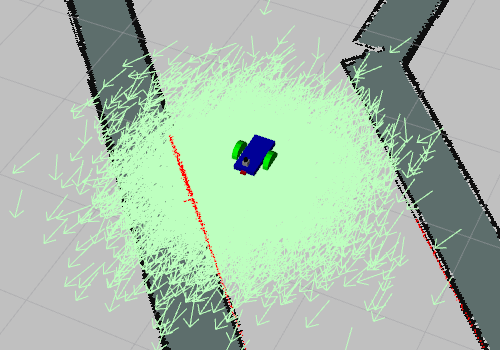
\includegraphics[height=4.5cm]{og_model_1}}
\captionof{figure}{Benchmark model before the localisation process has commenced. Note the distribution of green pose arrows around the robot indicating a high level of pose uncertainty.}
\end{minipage}
\hspace{1cm}
\begin{minipage}[t]{0.45\textwidth}
\centering
\frame{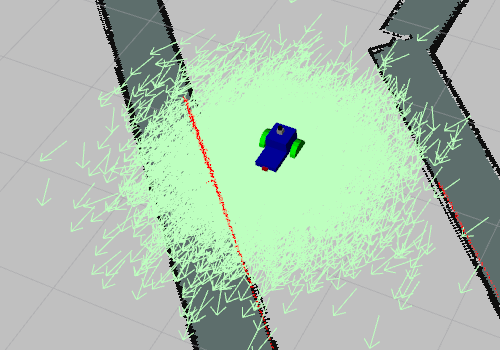
\includegraphics[height=4.5cm]{new_model_1}}
\captionof{figure}{Personal model before the localisation process has commenced. Note the distribution of green pose arrows around the robot indicating a high level of pose uncertainty.}
\end{minipage}

\vspace{1cm}

\begin{minipage}{0.45\textwidth}
\centering
\frame{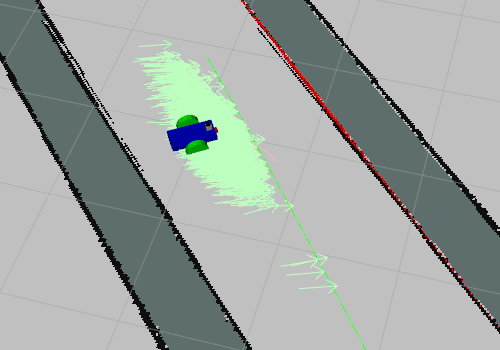
\includegraphics[height=4.5cm]{og_model_2}}
\captionof{figure}{Benchmark model navigating the environment as \texttt{amcl} localises the robot. The distribution of green arrows is beginning to converge on the correct pose.}
\end{minipage}
\hspace{1cm}
\begin{minipage}{0.45\textwidth}
\centering
\frame{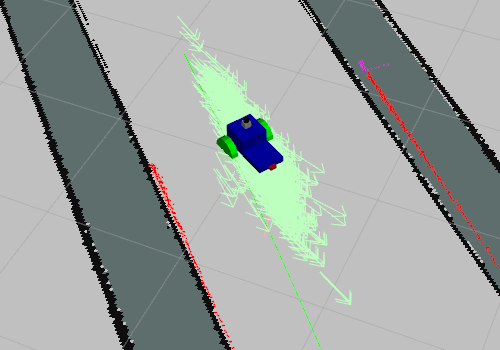
\includegraphics[height=4.5cm]{new_model_2}}
\captionof{figure}{Personal model navigating the environment as \texttt{amcl} localises the robot. The distribution of green arrows is beginning to converge on the correct pose.}
\end{minipage}

\vspace{1cm}

\begin{minipage}{0.45\textwidth}
\centering
\frame{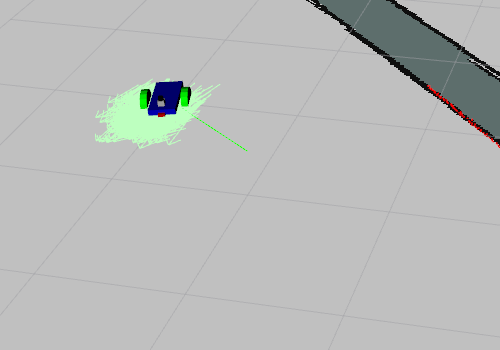
\includegraphics[height=4.5cm]{og_model_3}}
\captionof{figure}{Benchmark model at the goal location. The tight clustering of green arrows indicates particle convergence on true robot location for \texttt{amcl}}
\end{minipage}
\hspace{1cm}
\begin{minipage}{0.45\textwidth}
\centering
\frame{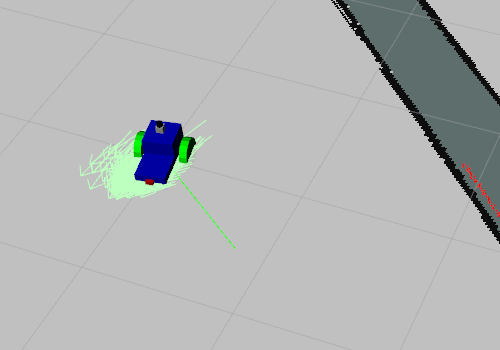
\includegraphics[height=4.5cm]{new_model_3}}
\captionof{figure}{Personal model at the goal location. The tight clustering of green arrows indicates particle convergence on true robot location for \texttt{amcl}}
\end{minipage}


\section{Conculsion}
Two robot models with differing body geometries and sensor locations were tested to determine the robustness of \texttt{amcl} and \texttt{move\_base} packages, used to implement MCL on a mobile robot platform. Experimental simulation provided some evidence that time taken to localise within an environment is not affected by changes to robot geometries and sensor locations, however, this may not be the case for algorithm stability and navigation path efficiency. The personal model appeared to experience reduced stability becoming stuck in the environment more often, but was able to navigate to the goal pose faster than the benchmark model. Ultimately these findings are inconclusive, and more experimental trials need to be undertaken to determine if observations were due to stochastic variation or not.


\bibliography{my_bib}
\bibliographystyle{ieeetr}

\end{document}